The theory of first order quasi-linear system is now applied to solid dynamics. First, the characteristic analysis of systems \eqref{eq:HPP_quasi-linear}, \eqref{eq:HE_quasilinear} and \eqref{eq:EP_quasilinear} is performed. Then by specializing the results to problems involving a linear elastic bar and a hyperelastic Saint-Venant-Kirchhoff medium, we shall see that different types of waves can propagate within a solid.

\subsection{Characteristic structure of solutions}
For the sake of simplicity studies of finite deformation and linearized geometrical frameworks will be condensed in this part by using a generic stress measure $\tens{S}$ and vectors written in the reference configuration. Furthermore, instead of studying multi-dimensional conservation laws systems, we will focus without loss of generality on conservative forms \eqref{eq:general_conservative} projected on an arbitrary direction $\vect{N}=\[\vect{e}_1,\vect{e}_2,\vect{e}_3\]$ \cite[p.425-426]{Leveque}. In this direction, the quasi-linear forms determined above are rewritten as:
\begin{equation}
  \label{eq:normal_quasi}
  \Qcb_t + \Jbsf \drond{\Qcb}{X_N} = \Scb
\end{equation}
where $X_N=\vect{X}\cdot\vect{N}$ and the \textit{Jacobian matrix} $\Jbsf = \Absf^\alpha N_\alpha$ of dimension $m$ arise. Hence, the characteristic analysis of system \eqref{eq:normal_quasi} is equivalent to that of linear combinations of matrices $\Absf^\alpha$. With the previous developments, the Jacobian matrix reads:
\begin{equation}
  \label{eq:jacobian_generic}
  \Jbsf=-\matrice{\tens{0}^2 & \frac{1}{\rho_0}\tens{I}\otimes \vect{N} \\  \tilde{\Hbb}\cdot\vect{N} & \tens{0}^4 }
\end{equation}
in which $\tilde{\Hbb}$ is either the hyperelastic or elastoplastic tangent modulus, or the elastic stifness tensor depending on the case considered. For general three-dimensional case, the characteristic structure of the problem is given by the $12$ eigenvalues $c_k$ and associated left eigenvectors $\Lcb^k$ of the Jacobian matrix:
\begin{equation}
  \label{eq:eigen_system}
  \vect{\Lc}^k\cdot \(\Jbsf - c_k \Ibsf\) = \vect{0}
\end{equation}
where $\Ibsf$ is the identity matrix and $\vect{\Lc}^k= \[ \vect{v}^K \: , \: \tens{S}^K \]$, with $\tens{S}$ standing for the suitable stress mesure. Thus, for non-null eigenvalues one gets:
\begin{subequations}
  \begin{alignat}{1}
    \label{eq:eigen_left_stress}
    & -\tens{S}^k:\(\tilde{\Hbb}\cdot  \vect{N}\) - c_k  \vect{v}^k =\vect{0} \\
    \label{eq:eigen_left_velo}
    & -\frac{1}{\rho_0}\vect{v}^k\otimes\vect{N} - c_k \tens{S}^k = \tens{0}
  \end{alignat}
\end{subequations}
Substitution of $\tens{S}$ obtained from \eqref{eq:eigen_left_velo} in \eqref{eq:eigen_left_stress} leads to:
\begin{equation}
  \label{eq:acoustic_eigen}
 (\vect{v}^k\otimes\vect{N}):\(\tilde{\Hbb}\cdot  \vect{N}\) - \rho_0\lambda^2_k \vect{v}^k = \tens{0}
\end{equation}
System \eqref{eq:acoustic_eigen} is the \textit{acoustic tensor} $A_{ij}=N_\alpha \tilde{H}_{i\alpha j \beta}  N_\beta$ left eigensystem which, due to the symmetry of $\tens{A}$ is equivalent to the right eigensystem:
\begin{equation}
  \label{eq:acoustic_eigen_system_lambda}
  \(  N_\alpha \tilde{H}_{i\alpha j \beta}  N_\beta - \rho_0 c_k^2 \delta_{ij} \) v_j^k =0
\end{equation}
or atlernatively with the eigenvalues $\omega_p$ and associated left eigenvectors of the acoustic tensor $\vect{l}^p\: \: (p=1,2,3)$:
\begin{equation}
  \label{eq:acoustic_eigen_system}
  \( \tens{A} - \omega_p \tens{I} \) \vect{l}^p = \vect{0}
\end{equation}
The condition for system \eqref{eq:normal_quasi} to be hyperbolic and have real eigenvalues and associated eigenvectors is thus ensured by the positive definiteness of the acoustic tensor, also known as the \textit{strong ellipticity} condition \cite{Foundation_of_elasticity}:
\begin{equation}
  \label{eq:strong_ellipticity}
  (\vect{m}\otimes \vect{N}): \tilde{\Hbb}: (\vect{m}\otimes \vect{N}) > 0 \quad \forall \vect{N},\vect{m} \in \Rbb^3 \: ; \: \vect{N},\vect{m} \ne \vect{0}
\end{equation}
If the condition holds, the acoustic tensor admits $3$ couples eigenvalues--eigenvectors $\{\omega_p,\vect{l}^p\}$ leading to $6$ couples $\{c_k,\Lcb^k\}$ for the Jacobian matrix, the $6$ other eigenvalues being null \cite{Kluth}. The couples $\{c_k,\Lcb^k\}$ are referred to as \textit{left characteristic fields}. The left eigenvectors associated to non-zero eigenvalues of the Jacobian matrix are obtained by using equation \eqref{eq:eigen_left_velo} so that the following $6$ eigenfields of quasi-linear form \eqref{eq:normal_quasi} can be defined:
\begin{equation}
  \label{eq:left_eigenfields}
    \left\lbrace \pm \sqrt{\frac{\omega_p}{\rho_0}} ; \quad \[\: \pm \rho_0\sqrt{\frac{\omega_p}{\rho_0}} \vect{l}^p , -\vect{l}^p\otimes \vect{N} \:\]  \right\rbrace ,\quad p=1,2,3
\end{equation}
At last, one has to find six independent left eigenvectors associated to the null eigenvalue of multiplicity $6$ by solving equation of \eqref{eq:eigen_left_stress} for the null eigenvalue:
\begin{equation}
  \label{eq:left_null_eigenvectors}
  \tens{S}^k:\(\tilde{\Hbb}\cdot  \vect{N}\) =\vect{0},\quad k=1,...,6
\end{equation}
Following the same procedure for right eigenvectors $\Rcb^k=\matrice{\vect{v}^k \\ \tens{S}^k}$, the Jacobian matrix right eigensystem reads:
\begin{subequations}
  \begin{alignat}{1}
    \label{eq:eigen_right_stress}
    & -\frac{1}{\rho_0}\tens{S}^k\cdot  \vect{N} - c_k  \vect{v}^k =\vect{0} \\
    \label{eq:eigen_right_velo}
    & -\tilde{\Hbb}:\(\vect{v}^k\otimes\vect{N}\) - c_k \tens{S}^k = \tens{0}
  \end{alignat}
\end{subequations}
which leads to the \textit{right eigen fields} associated to the non-null eigenvalues:
\begin{equation}
  \label{eq:right_eigenfields}
  \left\lbrace \pm \sqrt{\frac{\omega_p}{\rho_0}} ; \quad \[\: \pm \sqrt{\frac{\omega_p}{\rho_0}} \vect{l}^p , -\tilde{\Hbb}:\( \vect{l}^p\otimes \vect{N}\) \:\]  \right\rbrace ,\quad p=1,2,3
\end{equation}
In equation \eqref{eq:right_eigenfields}, $\{\omega_p,\vect{l}^p\}$ still denotes the eigenfields of the acoustic tensor. Moreover, the $6$ independent right eigenvectors associated to the zero eigenvalue required to complete the set of right characteristic fields must satisfy:
\begin{equation}
  \label{eq:right_null_eigenvectors}
  \tens{S}^k \cdot  \vect{N} =\vect{0},\quad k=1,...,6
\end{equation}

Note that since the right-hand side of equation \eqref{eq:normal_quasi} is not involved in the characteristic analysis, linear elasticity and elaso-viscoplasticity leads to the same characteristic structure. Furthermore, the specialization of characteristic equations \eqref{eq:PDEs_ODEs} to system \eqref{eq:normal_quasi} leads to:
\begin{equation}
  \label{eq:characteristic_equations_homogeneous}
  \Lcb^k \cdot d\Qcb = \vect{0},\quad k=1,...,6
\end{equation}
meaning that the solution is constant along each ray $\xi = x/t$ through the origin. Solutions $\Qcb(\xi)$ are then called \textit{similarity solutions} and allow to rewrite the quasi-linear form as:
\begin{equation}
  \label{eq:quasi-linear_similarity}
  -\frac{x}{t^2}\Qcb'(\xi) + \Jbsf \frac{1}{t}\Qcb'(\xi) = \vect{0} \quad \Rightarrow \quad \(\Jbsf- \xi \:\Ibsf \) \Qcb'(\xi) = \vect{0}
\end{equation}
By looking at characteristic curves $\xi=c_k$, system \eqref{eq:quasi-linear_similarity} implies that $\Qcb'$ is proportional to the right eigenvector $\Rcb^k$ and integration of $\Qcb'$ yields an \textit{integral curve} that is tangent at every point of the \textit{phase plane} $\(\Qcb_1,...,\Qcb_{m}\)$ to this eigenvector.

\boxe{USEFULL ?:
The notions highlighted so far will be illustrated in the two following sections. The method of characteristics will lead to:
\begin{itemize}
\item[(i)] the well-known solution to the \textit{Riemann problem} on a elastic bar
\item[(ii)] the development of the solution the Riemann problem of a hyperelastic Saint-Venant-Kirchhoff medium undergoing a one-dimensional strain state
\end{itemize}
Furthermore, the \textit{Rankine-Hugoniot condition} for discontinuous waves, and the concept of \textit{shock} and \textit{simple} waves will be introduced.}

\subsection{Linear problems}
\label{subsec:charac_Linear_problems}
A Riemann problem is a Cauchy problem composed of a hyperbolic system and piecewise constant initial data on both sides of an interface. In the arbitrary direction $\vect{n}=\[\vect{e}_1,\vect{e}_2,\vect{e}_3\]$, the Riemann problem reads:
\begin{equation}
  \label{eq:Riemann_problem}
  \begin{aligned}
  &\Qcb_t + \drond{\Fcb\cdot \vect{n}}{x_n} = \Scb, \\
  &\left\lbrace 
    \begin{aligned}
      & \Qcb(x_n,t=0) = \Qcb^L \quad \text{if } x_n< 0\\
      & \Qcb(x_n,t=0) = \Qcb^R \quad \text{if } x_n> 0
    \end{aligned}
    \right.
  \end{aligned}
\end{equation}

We consider a one-dimensional elastic medium of density $\rho$ undergoing one-dimensional stress and strain states within the infinitesimal framework: $\tens{\eps}=\eps\: \vect{e}_1\otimes \vect{e}_1$ ; $\tens{\sigma}=\sigma \:\vect{e}_1\otimes \vect{e}_1$, so that the bar hypothesis holds with $\vect{v}=v \vect{e}_1$. The Riemann problem consists then of problem \eqref{eq:Riemann_problem} for $\vect{n}=\vect{e}_1$ and $X_n=x$.

Neglecting body forces without loss of generality and introducing \textit{Yound's modulus E} such that $\sigma = E\eps$, conserved quantities and flux vector are:
\begin{equation*}
  \Qcb = \matrice{v \\ \sigma} \quad ; \quad \Fcb = \matrice{-\frac{1}{\rho}\sigma \\ -Ev}
\end{equation*}
The eigenvalues and left eigenvectors of the corresponding Jacobian matrix are:
\begin{equation*}
  % c_{1,2} = \mp \sqrt{\frac{E}{\rho}}=\pm c
  \left\lbrace
    \begin{aligned}
      & c_1=- \sqrt{\frac{\lambda+2\mu}{2\rho_0}\(3F^2-1\) }=-c\\
      & c_2= \sqrt{\frac{\lambda+2\mu}{2\rho_0}\(3F^2-1\) }=c
    \end{aligned}\right.
 \quad ; \quad \Lcb^p=\[\rho c_p \:,\: -1\] \quad ; \quad \Rcb^p=\matrice{1\\- \rho c_p } 
\end{equation*}

\subsubsection*{The method of characteristics}
The system of ODE along the characteristic curves, given by characteristic equations \eqref{eq:PDEs_ODEs}, is:
\begin{equation}
  \label{eq:elast_charac_equation}
  \Lcb^p \cdot d\Qcb = 0 \quad \Rightarrow
  \left\lbrace
    \begin{aligned}
      -& \rho c\: dv - d\sigma = 0\\
      & \rho c\: dv - d\sigma = 0
    \end{aligned} \right.
\end{equation}
Consider now a point $P$ of the ($x,t$) plane at which we are looking for the solution. Applying the method of characteristic, we trace the two characteristic straight lines starting from the $x$-axis (along which $\Qcb$ is given) and passing through $P$ (dashed lines in figure \ref{fig:elasticity_example}).  
\begin{figure}[h]
  \centering
  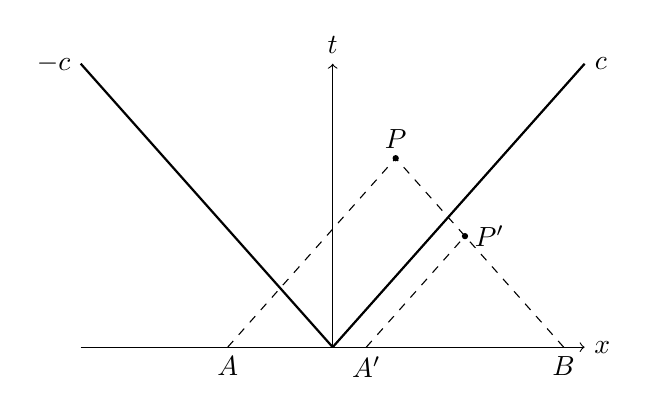
\begin{tikzpicture}[scale=0.8]
  \draw[->] (-4,0) -- (4.,0) node[right] {$x$};
  \draw[->] (0,0) -- (0,4.5) node[above] {$t$};
  \draw[thick] (0,0) -- (4.,4.5) node [right] {$c$};
  \draw[thick] (0,0) -- (-4.,4.5) node [left] {$-c$};
  \fill[black] (1.,3.) circle (0.05) node [above] {$P$};
  \draw[dashed] (1-8./3.,0.) node [below] {$A$}  -- (1.,3.);
  \draw[dashed] (1+8./3.,0.)node [below] {$B$}  -- (1.,3.);
  %% Intersection of positive solid line and negative dashed one
  %\fill[black] (0.5+12/9.,2.) circle (0.05) node [above] {$P'$};
  \fill[black] (2.10,1.762499) circle (0.05) node [right] {$P'$};
  \draw[dashed] (0.5333,0.) node [below] {$A'$}  -- (2.10,1.762499);
\end{tikzpicture}



%%% Local Variables:
%%% mode: latex
%%% TeX-master: "../../mainManuscript"
%%% End:

  \caption{Solution to Riemann problem \eqref{eq:Riemann_problem} for an elastic bar.}
  \label{fig:elasticity_example}
\end{figure}
Integration of characteristic equations \eqref{eq:elast_charac_equation} respectively along $AP$ and $BP$ yields:
\begin{equation}
  \label{eq:elastic_integral_curves}
  \left\lbrace
    \begin{aligned}
      -& \rho c \(v_P - v_A \) - \(\sigma_P - \sigma_A \) = 0\\
      & \rho c \(v_P - v_B \) - \(\sigma_P - \sigma_B \) = 0
    \end{aligned}
    \right.
\end{equation}
which solution is:
\begin{equation}
  \label{eq:elastic_solution_P}
  v_P = \frac{\sigma_B - \sigma_A}{2\rho c} + \frac{v_A+v_B}{2} \quad ; \quad \sigma_P = \rho c\frac{v_B - v_A}{2} + \frac{\sigma_A+\sigma_B}{2}
\end{equation}
On the other hand, the same procedure for point $P'$ leads to the solution:
\begin{equation}
  \label{eq:elastic_solution_Q}
  v_{P'} = \frac{\sigma_B - \sigma_{A'}}{2\rho c} + \frac{v_{A'}+v_B}{2} \quad ; \quad \sigma_{P'} = \rho c\frac{v_B - v_{A'}}{2} + \frac{\sigma_{A'}+\sigma_B}{2}
\end{equation}
With initial data given for the Riemann problem, it appears that $\Qcb_{A'}=\Qcb_{B}$ and hence, $\Qcb_{P'}=\Qcb_{R} \ne \Qcb_{P}$. Let's assume now that points $P$ and $P'$ are still on each side of the right characteristic straight line emanating from the origin but infinitely close to it. The previous results obviously hold along the characteristics so that a jump discontinuity propagates in the bar with speed $c$ The solutions of Riemann problem \eqref{eq:Riemann_problem} therefore consist in waves emanating from the origin of the $(x,t)$ plane. Across such discontinuous waves, the following condition is satisfied \cite{Toro}:
\begin{definition}
Given a system of hyperbolic conservation laws $\Qcb_t + \Fcb(\Qcb)_x=\vect{0}$ and a discontinuous wave solution of speed $s_i$ associated to the $i$th characteristic field, the \textbf{Rankine-Hugoniot condition} reads:
\begin{equation}
  \label{eq:rankine-hugoniot}
  \saut{ \Fcb} = s_i \saut{ \Qcb}
\end{equation}
where $\saut{\bullet}$ denotes the jump operator across the discontinuity.  
\end{definition}

\subsubsection*{Characteristic variables -- Waves solution}
Consider a quasi-linear form $\Qcb_t + \Jbsf \Qcb_x=\vect{0}$ of dimension $m$. 
By introducing a set of \textbf{characteristic variables} $\Pcb=\Rbsf^{-1}\Qcb$, where $\Rsf_{ij}=\Rc^j_i$ is the matrix of right eigenvectors, the quasi-linear form of system \eqref{eq:Riemann_problem} can be rewritten in terms of characteristic the variables:
\begin{equation*}
  \begin{aligned}
    &\drond{\Pc_i}{t} + c_i\drond{\Pc_i}{x} = 0 \\
    &\left\lbrace 
      \begin{aligned}
        & \Pc_i(x,t=0) = \Pc_i^L \quad \text{if } x< 0\\
        & \Pc_i(x,t=0) = \Pc_i^R \quad \text{if } x> 0
      \end{aligned}
    \right.
  \end{aligned}
\end{equation*}
\begin{figure}[h]
  \centering
  %\subfloat{\begin{tikzpicture}[scale=0.6]
  \draw[->] (-4,0) -- (4.,0) node[right] {$x$};
  \draw[->] (0,0) -- (0,4.5) node[above] {$t$};
  \draw[thick] (0,0) -- (4.,4) node [right] {$c_i$};
  % \fill[black] (1.,3.) circle (0.05) node [above] {$P$};
  % \fill[black] (2.10,1.762499) circle (0.05) node [right] {$P'$};
  \draw[dotted] (-4,1.)-- (0,1) node [above left] {$t_1$} --(4.,1);
  \draw[dotted] (-4,2.)-- (0,2) node [above left] {$t_2$} --(4.,2);
  \node[above left] at (0,0) {$t_0$};
\end{tikzpicture}

%%% Local Variables:
%%% mode: latex
%%% TeX-master: "../../mainManuscript"
%%% End:}
  %\subfloat{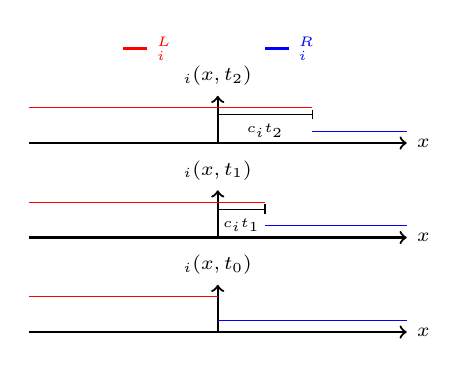
\begin{tikzpicture}[scale=0.6]
  %% t2
  \draw[->,thick] (0,0) -- (0,1) node [above] {\scriptsize$\Pc_i(x,t_2)$};
  \draw[->,thick] (-4,0) -- (4,0) node [right] {\scriptsize$x$};
  \draw[Blue] (2,0.25) -- (4,0.25);
  \draw[Red] (-4,0.75) -- (2,0.75);
  \draw (0,0.6)--(2,0.6) node [midway, below] {\tiny $c_it_2$};
  \draw (2,0.5)--(2,0.7);
  %% t1
  \draw[->,thick] (0,-2) -- (0,-1) node [above] {\scriptsize$\Pc_i(x,t_1)$};
  \draw[->,thick] (-4,-2) -- (4,-2) node [right] {\scriptsize$x$};
  \draw[Blue] (1,0.25-2) -- (4,0.25-2);
  \draw[Red] (-4,0.75-2) -- (1,0.75-2);
  \draw (0,0.6-2)--(1,0.6-2) node [midway, below] {\tiny $c_it_1$};
  \draw (1,0.5-2)--(1,0.7-2);
  %% t0
  \draw[->,thick] (0,-4) -- (0,-3) node [above] {\scriptsize$\Pc_i(x,t_0)$};
  \draw[->,thick] (-4,-4) -- (4,-4) node [right] {\scriptsize$x$};
  \draw[Blue] (0,0.25-4.) -- (4,0.25-4.);
  \draw[Red] (-4,0.75-4.) -- (0,0.75-4.);
  %% legend
  \draw[thick,Red] (-2.,2.) -- (-1.5,2.) node [right] {\scriptsize$\Pc_i^L$};
  \draw[thick,Blue] (1,2.) -- (1.5,2.) node [right] {\scriptsize$\Pc_i^R$};
\end{tikzpicture}
%%% Local Variables:
%%% mode: latex
%%% TeX-master: "../../mainManuscript"
%%% End:}
  \subcaptionbox*{}[0.45\linewidth]{\begin{tikzpicture}[scale=0.6]
  \draw[->] (-4,0) -- (4.,0) node[right] {$x$};
  \draw[->] (0,0) -- (0,4.5) node[above] {$t$};
  \draw[thick] (0,0) -- (4.,4) node [right] {$c_i$};
  % \fill[black] (1.,3.) circle (0.05) node [above] {$P$};
  % \fill[black] (2.10,1.762499) circle (0.05) node [right] {$P'$};
  \draw[dotted] (-4,1.)-- (0,1) node [above left] {$t_1$} --(4.,1);
  \draw[dotted] (-4,2.)-- (0,2) node [above left] {$t_2$} --(4.,2);
  \node[above left] at (0,0) {$t_0$};
\end{tikzpicture}

%%% Local Variables:
%%% mode: latex
%%% TeX-master: "../../mainManuscript"
%%% End:}
  \subcaptionbox*{}[0.45\linewidth]{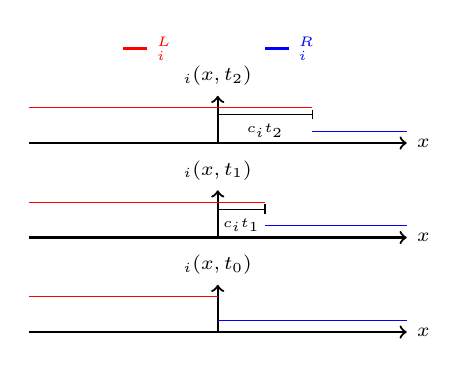
\begin{tikzpicture}[scale=0.6]
  %% t2
  \draw[->,thick] (0,0) -- (0,1) node [above] {\scriptsize$\Pc_i(x,t_2)$};
  \draw[->,thick] (-4,0) -- (4,0) node [right] {\scriptsize$x$};
  \draw[Blue] (2,0.25) -- (4,0.25);
  \draw[Red] (-4,0.75) -- (2,0.75);
  \draw (0,0.6)--(2,0.6) node [midway, below] {\tiny $c_it_2$};
  \draw (2,0.5)--(2,0.7);
  %% t1
  \draw[->,thick] (0,-2) -- (0,-1) node [above] {\scriptsize$\Pc_i(x,t_1)$};
  \draw[->,thick] (-4,-2) -- (4,-2) node [right] {\scriptsize$x$};
  \draw[Blue] (1,0.25-2) -- (4,0.25-2);
  \draw[Red] (-4,0.75-2) -- (1,0.75-2);
  \draw (0,0.6-2)--(1,0.6-2) node [midway, below] {\tiny $c_it_1$};
  \draw (1,0.5-2)--(1,0.7-2);
  %% t0
  \draw[->,thick] (0,-4) -- (0,-3) node [above] {\scriptsize$\Pc_i(x,t_0)$};
  \draw[->,thick] (-4,-4) -- (4,-4) node [right] {\scriptsize$x$};
  \draw[Blue] (0,0.25-4.) -- (4,0.25-4.);
  \draw[Red] (-4,0.75-4.) -- (0,0.75-4.);
  %% legend
  \draw[thick,Red] (-2.,2.) -- (-1.5,2.) node [right] {\scriptsize$\Pc_i^L$};
  \draw[thick,Blue] (1,2.) -- (1.5,2.) node [right] {\scriptsize$\Pc_i^R$};
\end{tikzpicture}
%%% Local Variables:
%%% mode: latex
%%% TeX-master: "../../mainManuscript"
%%% End:}
  \caption{Solution to linear advection equation on the quantity $\Pc_i$ with characteristic speed $c_i$.}
  \label{fig:advection}
\end{figure}
with $\Csf_{ij}=c_i\delta_{ij}$, the matrix of eigenvalues so that $\Jsf_{ij} \Rc^j_k = \Rc^k_i\Csf_{kj}$. The solution of this problem is straightforward since it corresponds to a superposition of scalar linear advection equations namely, the initial profil $\Pc_i(x,t=0)$ simply propagates with speed $c_i$ as depicted in figure \ref{fig:advection}. Thus, at a given point $(x,t)$, the solution $\Pc_i(x,t)$ is simply given by tracing backward the characteristic of slope $c_i$ passing through this point to the $x$-axis, that is: $\Pc_i(x,t)=\Pc_i(x-c_it,0)$. 
The vector $\Qcb$ is then determined by inverting the relation:
\begin{equation}
  \label{eq:Q_expansion}
  \Qcb(x,t) = \sum_{i=1}^m \Rcb^i \Pc_i(x-c_it,0) \quad \Rightarrow
  \left\lbrace
    \begin{aligned}
      & \Qcb(x<0,0)=\Qcb^L=\sum_{i=1}^{m}\Rcb^i \Pc_i^L\\
      & \Qcb(x>0,0)=\Qcb^R= \sum_{i=1}^{m}\Rcb^i \Pc_i^R
    \end{aligned}
    \right.
\end{equation}
Equation \eqref{eq:Q_expansion} is an eigenvector expansion with coefficients $\Pc_i^{R,L}$ from which we see that $\Qcb$ is a superposition of $m$ waves, each of which having the shape $\Rcb^i \Pc_i(x,0)$. Noticing that for given values of $x$ and $t$, there exists one characteristic $I$ such that $x-c_I t >0$ and $x-c_{I+1} t <0$, equation \eqref{eq:Q_expansion} can be rewritten:
\begin{equation}
  \label{eq:Q_expansion_sides}
  \Qcb = \sum_{i=1}^I \Rcb^i \Pc_i^R + \sum_{i=I+1}^m \Rcb^i \Pc_i^L
\end{equation}
or, introducing the expansions of initial data \eqref{eq:Q_expansion_sides}:
\begin{align}
  &\Qcb = \sum_{i=1}^m \Rcb^i \Pc_i^R - \sum_{i=I+1}^m \Rcb^i \(\Pc_i^R - \Pc_i^L\)= \Qcb^R - \sum_{i=I+1}^m \Rcb^i \(\Pc_i^R - \Pc_i^L\) \\
  &\Qcb= \sum_{i=1}^{m}\Rcb^i \Pc_i^L + \sum_{i=1}^I \Rcb^i \(\Pc_i^R - \Pc_i^L\)= \Qcb^L + \sum_{i=1}^I \Rcb^i \(\Pc_i^R - \Pc_i^L\) 
\end{align}
Those equations are equivalent to jump conditions across mutliple discontinuous waves:
\begin{align}
  \label{eq:jump_star_R}
  &  \Qcb-\Qcb^R = -\sum_{i=I+1}^{m} \Rcb^i\delta^i \\
  \label{eq:jump_star_L}
  &  \Qcb-\Qcb^L = \sum_{i=1}^{I} \Rcb^i\delta^i \\
\end{align}
where $\Qcb(x,t)$ is the state lying in the region of the ($x,t$) plane delimited by the $I$th and $(I+1)$th characteristics, and $\Rcb^i\delta^i$ the jump carried by the $i$th wave. The coefficients $\delta^i=\Pc_i^R - \Pc_i^L$ are called the \textit{wave strengths} and can be computed from the expensions of initial conditions by solving:
\begin{equation}
  \label{eq:delta_system}
  \Qcb^R-\Qcb^L=\sum_{i=1}^{m}\Rcb^i \delta^i=\Rbsf \vect{\delta}
\end{equation}
Writing $\Qcb^R-\Qcb^L=\Delta \Qcb$, linear systems of dimension $2$ lead to wave strengths coefficients:
\begin{equation}
  \label{eq:wave_strengths}
  \vect{\delta} = \frac{1}{\Rc_1^2-\Rc^1_1}\matrice{\Rc^2_1 \Delta \Qc_2 - \Delta \Qc_1 \\ \Delta \Qc_1 - \Rc_1^1\Delta \Qc_1}
\end{equation}
which, combined to equation \eqref{eq:jump_star_L}, yields the solution found by using the method of characteristics \eqref{eq:elastic_solution_P} for linear elasticity:
\begin{equation}
  \label{eq:solution_charac_variables}
  \Qcb = \Qcb^L +\Rcb^1 \delta^1 = \matrice{\frac{\sigma_B - \sigma_A}{2\rho c} + \frac{v_A+v_B}{2} \\ \rho c\frac{v_B - v_A}{2} + \frac{\sigma_A+\sigma_B}{2}} 
\end{equation}

\subsection{Non-linear problems}
\label{subsec:charac_nonlinear_problems}
We now consider a hyperelastic medium made of a Saint-Venant-Kirchhoff material, infinite in directions $\vect{e}_2$ and $\vect{e}_3$, and semi-infinite in direction $\vect{e}_1$ (\textit{i.e. $x_1 \in [0,+\infty[$}). This medium suddenly undergoes a load at $(X_1=X=0,t=0)$ in direction $\vect{e}_1$ so that the deformation gradient and the PK1 tensor are respectively:
\begin{align*}
  &\tens{F}=F\vect{e}_1\otimes\vect{e}_1 + \vect{e}_2\otimes\vect{e}_2 + \vect{e}_3\otimes\vect{e}_3 \\
  & \tens{\Pi}=\Pi_{11}\vect{e}_1\otimes\vect{e}_1 + \Pi_{22}\(\vect{e}_2\otimes\vect{e}_2 + \vect{e}_3\otimes\vect{e}_3 \)
\end{align*}
which corresponds to a plane wave solution. We assume that $F(0,t)=\bar{F}$ is given, leading to a \textit{Picard problem} involving both initial and boundary conditions with neglected body forces:
\begin{equation}
  \label{eq:Picard_problem}
  \begin{aligned}
  &\Qcb_t + \drond{\Fcb\cdot \vect{X}}{X_N} = \vect{0}, \\
  &\left\lbrace 
    \begin{aligned}
      & \Qcb(X_N,t=0) = \Qcb^R \quad \text{if } X_N> 0 \\
      & F(0,t) = \bar{F} 
    \end{aligned}
    \right.
  \end{aligned}
\end{equation}
with $\vect{N}=\vect{e}_1$ and:
\begin{equation*}
 \Qcb = \matrice{v \\ F} \quad ; \quad \Fcb = \matrice{-\frac{1}{\rho_0}\Pi \\ -v}
\end{equation*}
where $\Pi=\Pi_{11}$. Since the tangent modulus and the acoustic tensor of Saint-Venant-Kirchhoff model \eqref{eq:SVK_tangent},\eqref{eq:SVK_acoustic} depend on the deformation gradient, the quasi-linear form: $\Qcb_t + \drond{\Fcb}{\Qcb}\drond{\Qcb}{X}=\vect{0}$ is more convenient. The Jacobian matrix is then:
\begin{equation}
  \label{eq:quasi_SVK}
  \Jbsf=\drond{\Fcb}{\Qcb}=-\matrice{0 & \frac{H_{1111}}{\rho_0} \\ 1 & 0}
\end{equation}
which leads to the characteristic fields:
\begin{equation}
  \label{eq:SVK_charac_fields}
  \left\lbrace
    \begin{aligned}
      & c_1=- \sqrt{\frac{\lambda+2\mu}{2\rho_0}\(3F^2-1\) }\\
      &c_2= \sqrt{\frac{\lambda+2\mu}{2\rho_0}\(3F^2-1\) }
    \end{aligned}\right.
 \quad ; \quad \Lcb^p=\[1\:,\:- c_p \] \quad ; \quad \Rcb^p=\matrice{- c_p \\1} 
\end{equation}

\begin{remark}
  \label{rq:hyperbolicity_limit_SVK}
  The non-linear flux function of SVK model yields characteristic fields depending on the strain state and possibly complex celerities leading to a loss of hyperbolicity of the problem for $F<\sqrt{\frac{1}{3}}$.
\end{remark}

Initial and boundary conditions have an influence on the characteristic structure of the solution due to the dependence of characteristic speeds on the deformation gradient. Indeed, if initial data are given so that $\bar{F} > F_R$, the resulting characteristic speeds satisfy $c_2(\bar{F})>c_2(F_R)$ leading to characteristics colliding in the right region of the ($x,t$) plane (figure \ref{fig:Picard_problem}\subref{subfig:2S}). On the other hand, $\bar{F} < F_R$ yields characteristic moving away from each other in the right region according to $c_2(\bar{F})<c_2(F_R)$ (figure \ref{fig:Picard_problem}\subref{subfig:2R}). Those two situations, respectively corresponding to a shock wave and a simple wave, will be studied in what follows. \todo{\cite{Leveque} and shallow water equations}
\begin{figure}[h!]
  \centering
  % \begin{subfigure}[t]{}%{.49\textwidth}
  %   \centering
  %   \caption{Right-going shock wave}\label{subfig:2S}
  %   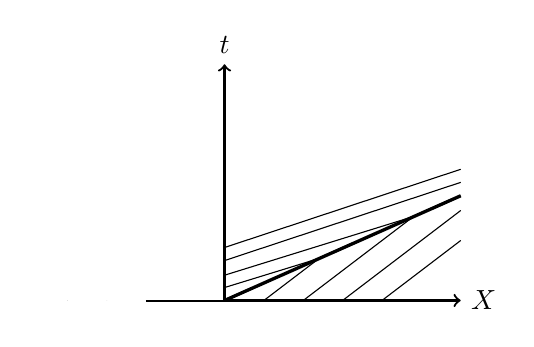
\begin{tikzpicture}
  \draw[->,thick] (-1,0) -- (3,0) node[right] {$X$};
  \draw[->,thick](0,0) -- (0,3) node[above] {$t$};
  \draw(-0.5,0.01) -- (1.20,0.533333) ;
  \draw(-1,0.01) -- (2.40,1.066) ;
  \draw(-1.5,0.01) -- (3,1.5) ;
  \draw(-2,0.01) -- (3,1.666) ;
  %%%%%%%%% 
  \draw(0.5,0) -- (1.20,0.533333) ;
  \draw(1.,0) -- (2.40,1.066) ;
  \draw(1.5,0) -- (3,1.14285) ;
  \draw(2.0,0) -- (3,0.7619) ;
  \draw[very thick] (0,0) -- (3,1.33);
  \fill[white] (-2.5,2.5) rectangle (-0.015,0.01);
  \fill[white] (-2.,0) rectangle (-1.,0.1);
\end{tikzpicture}
  % \end{subfigure}
  % \begin{subfigure}[t]{}%{.49\textwidth}
  %   \centering
  %   \caption{Right-going rarefaction wave}\label{subfig:2R}
  %   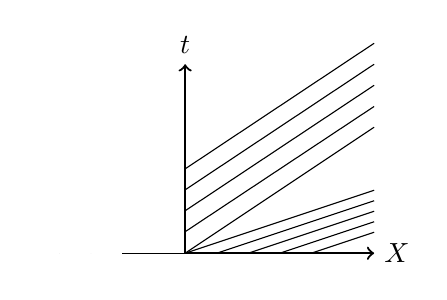
\begin{tikzpicture}[scale=0.8]
  \draw[->,thick] (-1,0) -- (3,0) node[right] {$X$};
  \draw[->,thick](0,0) -- (0,3) node[above] {$t$};
  \draw(0,0) -- (3,2) ;
  \draw(-0.5,0.01) -- (3,2.33) ;
  \draw(-1,0.01) -- (3,2.666) ;
  \draw(-1.5,0.01) -- (3,3) ;
  \draw(-2,0.01) -- (3,3.333) ;
  \draw(0,0) -- (3,1) ;
  \draw(0.5,0) -- (3,0.833) ;
  \draw(1,0) -- (3,0.666) ;
  \draw(1.5,0) -- (3,0.5) ;
  \draw(2,0) -- (3,0.333);
  \fill[white] (-2.5,2.5) rectangle (-0.015,0.01);
  \fill[white] (-2.,0) rectangle (-1.,0.1);
\end{tikzpicture}
  % \end{subfigure}
  \subcaptionbox{Right-going shock wave\label{subfig:2S}}{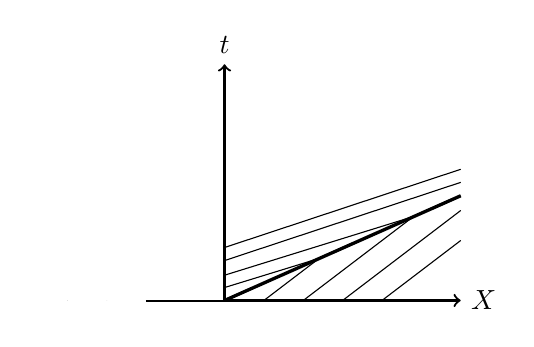
\begin{tikzpicture}
  \draw[->,thick] (-1,0) -- (3,0) node[right] {$X$};
  \draw[->,thick](0,0) -- (0,3) node[above] {$t$};
  \draw(-0.5,0.01) -- (1.20,0.533333) ;
  \draw(-1,0.01) -- (2.40,1.066) ;
  \draw(-1.5,0.01) -- (3,1.5) ;
  \draw(-2,0.01) -- (3,1.666) ;
  %%%%%%%%% 
  \draw(0.5,0) -- (1.20,0.533333) ;
  \draw(1.,0) -- (2.40,1.066) ;
  \draw(1.5,0) -- (3,1.14285) ;
  \draw(2.0,0) -- (3,0.7619) ;
  \draw[very thick] (0,0) -- (3,1.33);
  \fill[white] (-2.5,2.5) rectangle (-0.015,0.01);
  \fill[white] (-2.,0) rectangle (-1.,0.1);
\end{tikzpicture}}
  \subcaptionbox{Right-going simple wave\label{subfig:2R}}{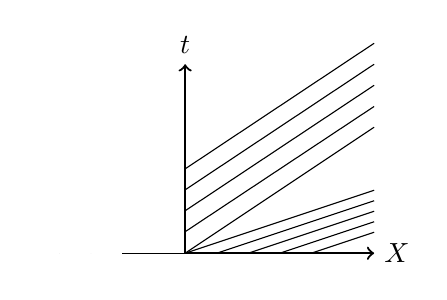
\begin{tikzpicture}[scale=0.8]
  \draw[->,thick] (-1,0) -- (3,0) node[right] {$X$};
  \draw[->,thick](0,0) -- (0,3) node[above] {$t$};
  \draw(0,0) -- (3,2) ;
  \draw(-0.5,0.01) -- (3,2.33) ;
  \draw(-1,0.01) -- (3,2.666) ;
  \draw(-1.5,0.01) -- (3,3) ;
  \draw(-2,0.01) -- (3,3.333) ;
  \draw(0,0) -- (3,1) ;
  \draw(0.5,0) -- (3,0.833) ;
  \draw(1,0) -- (3,0.666) ;
  \draw(1.5,0) -- (3,0.5) ;
  \draw(2,0) -- (3,0.333);
  \fill[white] (-2.5,2.5) rectangle (-0.015,0.01);
  \fill[white] (-2.,0) rectangle (-1.,0.1);
\end{tikzpicture}}
 \caption{Solutions to Picard problem \eqref{eq:Picard_problem} depending on initial and boundary data.}
  \label{fig:Picard_problem}
\end{figure}

\subsubsection*{Shock waves}
By applying the method of characteristics between the $x$-axis and an intersection point of two characteristic straight lines allows to show that a shock wave carry a jump discontinuity of the conserved quantities vector and hence, satisfy the Rankine-Hugoniot condition \eqref{eq:rankine-hugoniot} where the shock speed $s_i$ is to be defined. According to Rankine-Hugoniot conditions, those states obey:
\begin{align}
  \label{eq:RH_velocity}
  & -\frac{1}{\rho_0}\(\bar{\Pi} - \Pi_R \) = s \( \bar{v} - v_R \)\\
  \label{eq:RH_F}
  & - \( \bar{v}-v_R\)=s\( \bar{F} - F_R\)
\end{align}
For the sake of generality, $\bar{F}$ is considered as an unknown so that a relation connecting $\Qcb^R$ to a set of solutions $\Qcb$ through a shock wave can be developed.

Substitution of $s$ from equation \eqref{eq:RH_F} and introduction in equation \eqref{eq:RH_velocity} where $\Pi=\frac{\lambda+2\mu}{2}\(F^3-F\)$ yield:
\begin{align}
  \label{eq:shock_speed}
  & s=-\frac{v-v_R}{F - F_R}\\
  \label{eq:v_jump}
  & v-v_R= \pm \sqrt{\frac{\lambda+2\mu}{2\rho_0}(F-F_R)\[ F^3-F - (F_R^3-F_R)\]}
\end{align}
In addition to the Rankine-Hugoniot condition, the \textit{Lax entropy condition} stating that characteristic curves collide in a shock wave must be satisfied \cite[p.268]{Leveque}:
\begin{equation}
  \label{eq:Lax_entropy}
  \lambda(F)<s<\lambda(F_R)
\end{equation}
For a Saint-Venant-Kirchhoff material, the Lax condition leads to $F > F_R$ ensuring thus that the square root in equation \eqref{eq:v_jump} is real.


Equation \eqref{eq:v_jump} yields two families of curves in the phase plane, one of which is expected to identify with the jump conditions derived for the linear case \eqref{eq:jump_star_R} when considering an infinitesimal jump (\textit{i.e. $F=F_R+\epsilon$ with $\epsilon \rightarrow 0$}). Thus, equation \eqref{eq:v_jump} reads:
\begin{equation}
  \label{eq:linearization}
  v-v_R= \pm \sqrt{\frac{\lambda+2\mu}{2\rho_0}\epsilon\[ (F_R+\epsilon)^3-(F_R+\epsilon) - (F_R^3-F_R)\]}
\end{equation}
where, with $\epsilon \rightarrow 0$:
\begin{equation*}
  (F_R+\epsilon)^3\approx F_R^3(1+\frac{3\epsilon}{F_R})
\end{equation*}
and hence,
\begin{equation*}
  \matrice{v \\ F}=\matrice{v_R \\ F_R} + \epsilon \matrice{1 \\\pm \sqrt{\frac{\lambda+2\mu}{2\rho_0}\[ 3F_R^2-1\]}}
\end{equation*}
Hence, the \textit{minus} sign yields the linearized expression \eqref{eq:jump_star_R} for a right-going shock, the \textit{plus} sign holds, on the other hand, for left-going shocks. Finally, the Rankine-Hugoniot condition across a left-going shock and a right-going shock respectively yields:
\begin{align}
  \label{eq:left-going_shock}
  &v-v_L= \sqrt{\frac{\lambda+2\mu}{2\rho_0}(F-F_L)\[ F^3-F - (F_L^3-F_L)\]} \\
  \label{eq:right-going_shock}
  &v-v_R= -\sqrt{\frac{\lambda+2\mu}{2\rho_0}(F-F_R)\[ F^3-F - (F_R^3-F_R)\]}
\end{align}

\subsubsection*{Simple waves}
In order to study the evolution of fields within the void region in figure \ref{fig:Picard_problem}\subref{subfig:2R}, let's write the left-going characteristic equation through it with $\Lcb^1=[1,-c_1]$:
\begin{equation}
  \label{eq:SVK_rarefaction}
  dv -c_1  dF = 0 %+\sqrt{\frac{\lambda + 2\mu}{2\rho_0}\(3F^2-1\)}
\end{equation}

\begin{remark}
  If one was seeking a similarity solution in this region, the conserved quantities vector would be looked for so that $\Qcb'(x/t)$ is proportional to the right eigenvector $\Rcb^2$ asrequired by equation \eqref{eq:quasi-linear_similarity}. By denoting the ray $\xi=x/t$, this proportionality condition is:
  \begin{equation*}
    \matrice{\ddroit{v}{\xi} \\ \ddroit{F}{\xi}} = \matrice{ -c_2 \\ 1}
  \end{equation*}
  Combining \todo{Caution to $\alpha(\xi)$ \cite{Leveque}} these equations and noting that $c_2=-c_1$ allows to recover equation \eqref{eq:SVK_rarefaction}:
  \begin{equation}
    \label{eq:rarefaction}
    \begin{aligned}
      & dv -c_1 d\xi = 0\\
      & dF = d\xi
    \end{aligned}
  \end{equation}
Hence, the structure depicted in figure \ref{fig:Picard_problem}\subref{subfig:2R} corresponds to a rarefaction wave. Fields evolve smoothly within the void region according to equations \eqref{eq:rarefaction}, leading to a characteristic fan since $c_2=c_2(F)$ and $F$ decreases from $F_R$ to $\bar{F}$.
\end{remark}


As for shock waves, the complete set of states $\Qcb$ connected to $\Qcb^R$ through a rarefaction wave will be derived. To do so, the following change of variable is introduced: $F \mapsto ch(x)/\sqrt{3}$, so that equation \eqref{eq:SVK_rarefaction} becomes:
\begin{equation}
  \label{eq:charac_equation_sh}
  dv=-\sqrt{\frac{\lambda + 2\mu}{6\rho_0}}sh(x)^2 dx
\end{equation}
where, the hyperbolic cosine $ch(x)$ and sine $sh(x)$ satisfy: $ch(x)^2-sh(x)^2=1$. Equation \eqref{eq:charac_equation_sh} can be easily integrated with the exponential form of hyperbolic sine: $sh(x)=\frac{e^x - e^{-x}}{2}$. Thus, one gets:
\begin{equation*}
  v-v_R=-\frac{1}{4}\sqrt{\frac{\lambda + 2\mu}{6\rho_0}}\[sh(2x)-2x -(sh(2x_R)-2x_R)\]
\end{equation*}
At last, the inverse change of variable:
\begin{align*}
  &sh(2x)=2ch(x)sh(x)=2\sqrt{3}F\sqrt{3F^2-1} \\
  &2x=2\arg\(ch(\sqrt{3}F)\)=2\ln\(\sqrt{3}F + \sqrt{3F^2-1}\)
\end{align*}
yields the relation:
\begin{equation}
  \label{eq:integral_curve_right}
  v-v_R=-\sqrt{\frac{\lambda + 2\mu}{24\rho_0}}\[\sqrt{3}\(F\sqrt{3F^2-1} -F_R\sqrt{3F_R^2-1}\)-\ln\(\frac{\sqrt{3}F + \sqrt{3F^2-1}}{\sqrt{3}F_R + \sqrt{3F_R^2-1}}\) \]
\end{equation}
In a similar manner, the following condition must hold through a left-going rarefaction wave:
\begin{equation*}
  dv -c_2  dF = 0
\end{equation*}
which leads to:
\begin{equation}
  \label{eq:integral_curve_left}
  v-v_L=\sqrt{\frac{\lambda + 2\mu}{24\rho_0}}\[\sqrt{3}\(F\sqrt{3F^2-1} -F_L\sqrt{3F_L^2-1}\)-\ln\(\frac{\sqrt{3}F + \sqrt{3F^2-1}}{\sqrt{3}F_L + \sqrt{3F_L^2-1}}\) \]
\end{equation}


\subsubsection*{Solution of the Riemann problem}
Now the solution to Picard's problems have been derived, the solution of the Riemann problem can be developed. Once again, the problem is formulated as:
\begin{equation}
  \begin{aligned}
    &\Qcb_t + \drond{\Fcb\cdot \vect{N}}{X_N} = \vect{0}, \\
    &\left\lbrace 
      \begin{aligned}
        & \Qcb(X_N,t=0) = \Qcb^L \quad \text{if } X_N< 0\\
        & \Qcb(X_N,t=0) = \Qcb^R \quad \text{if } X_N> 0
      \end{aligned}
    \right.
  \end{aligned}
\end{equation}
As for the Picard problem, initial conditions influence the characteristic structure of the solution. Indeed, if initial conditions are given such that $F_L<F_R$, left-going characteristics will collide while right-going ones will move away from one another (see figure \ref{fig:RP_solution}\subref{subfig:1S2R}). In that case, the first and second characteristic fields will respectively be refered to as a \textit{1-shock} and a \textit{2-rarefaction}. Conversely, if $F_L>F_R$, the solution will correspond to a \textit{1-rarefaction} and a \textit{2-shock} (figure \ref{fig:RP_solution}\subref{subfig:1R2S}). 

\begin{figure}[h]
  \centering
  % \begin{subfigure}[t]{0.49\linewidth}
  %   \centering
  %   \caption{$F_L < F_R$\label{subfig:1S2R}}
  %   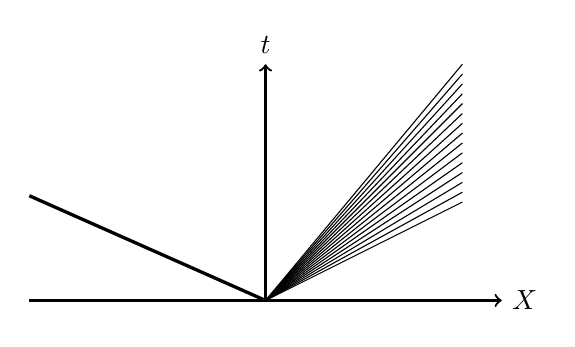
\begin{tikzpicture}
  \draw[->,thick] (-3,0) -- (3,0) node[right] {$X$};
  \draw[->,thick](0,0) -- (0,3) node[above] {$t$};
  %% Shock wave
  \draw[very thick] (0,0) -- (-3,1.33);
  %% Rarefaction wave
  \foreach \x in {0.5,0.55,...,1.25}
  \draw(0,0) -- (2.5,2.5*\x) ;
\end{tikzpicture}
  % \end{subfigure}
  % \begin{subfigure}[t]{0.49\linewidth}
  %   \centering
  %   \caption{$F_L > F_R$\label{subfig:1R2S}}
  %   \input{chapter2/pgfFigures/1R2S}
  % \end{subfigure}
  \subcaptionbox{$F_L < F_R$\label{subfig:1S2R}}{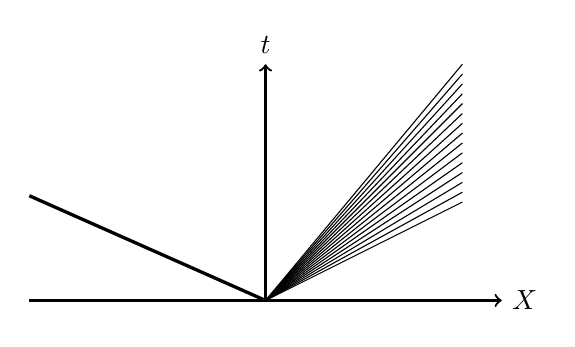
\begin{tikzpicture}
  \draw[->,thick] (-3,0) -- (3,0) node[right] {$X$};
  \draw[->,thick](0,0) -- (0,3) node[above] {$t$};
  %% Shock wave
  \draw[very thick] (0,0) -- (-3,1.33);
  %% Rarefaction wave
  \foreach \x in {0.5,0.55,...,1.25}
  \draw(0,0) -- (2.5,2.5*\x) ;
\end{tikzpicture}}
  \subcaptionbox{$F_L > F_R$\label{subfig:1R2S}}{\input{chapter2/pgfFigures/1R2S}}
  \caption{General wave patterns arrising in the solution to Riemann problem depending on intial data. (a): 1-shock, 2-rarefaction. (b): 1-rarefaction, 2-shock.}
  \label{fig:RP_solution}
\end{figure}

For the 1-shock,2-rarefaction solution one then seeks a state $\Qcb^*$ that is connected to $\Qcb^L$ and $\Qcb^R$ through respectively a shock wave and a rarefaction wave. Hence, $\Qcb^*$ must satisfy equations \eqref{eq:left-going_shock} and \eqref{eq:integral_curve_right}, namely:
\begin{equation}
  \label{eq:1S2R_solution}
  \left\lbrace
  \begin{aligned}
    &v_*-v_L= \sqrt{\frac{\lambda+2\mu}{2\rho_0}(F_*-F_L)\[ F_*^3-F_* - (F_L^3-F_L)\]} \\
    &v_*-v_R=-\sqrt{\frac{\lambda + 2\mu}{24\rho_0}}\[\sqrt{3}\(F_*\sqrt{3F_*^2-1} -F_R\sqrt{3F_R^2-1}\)-\ln\(\frac{\sqrt{3}F_* + \sqrt{3F_*^2-1}}{\sqrt{3}F_R + \sqrt{3F_R^2-1}}\) \]
  \end{aligned}
  \right.
\end{equation}
Analogously, the 1-rarefaction,2-shock solution is given by the solution of equations \eqref{eq:integral_curve_left} and \eqref{eq:right-going_shock}:
\begin{equation}
  \label{eq:1R2S_solution}
  \left\lbrace
  \begin{aligned}
    &v_*-v_L=\sqrt{\frac{\lambda + 2\mu}{24\rho_0}}\[\sqrt{3}\(F_*\sqrt{3F_*^2-1} -F_L\sqrt{3F_L^2-1}\)-\ln\(\frac{\sqrt{3}F_* + \sqrt{3F_*^2-1}}{\sqrt{3}F_L + \sqrt{3F_L^2-1}}\) \]\\
    &v_*-v_R= -\sqrt{\frac{\lambda+2\mu}{2\rho_0}(F_*-F_R)\[ F_*^3-F_* - (F_R^3-F_R)\]}
  \end{aligned}
  \right.
\end{equation}
\begin{figure}[h!]
  \centering
  {\input{chapter2/pgfFigures/1S2R_solution}\phantomsubcaption \label{subfig:1S2R_curves}}
  {\input{chapter2/pgfFigures/1R2S_solution}\phantomsubcaption  \label{subfig:1R2S_curves}}
  \caption{Set of connected states $\Qcb$ to initial data through shock and rarefaction waves with $v_L=v_R=0$ in both cases: (a) 1-shock, 2-rarefaction solution ; (b) 1-rarefaction, 2-shock.}
  \label{fig:solutions_RP}
\end{figure} 
Once one of this system is solved, the solution $\Qcb$ is known everywhere except inside the rarefaction fan. Nevertheless, in this region $\Qcb$ only varies with the ray $\xi=c_i(F)$ and hence, the solution inside an $i$-rarefaction wave satisfies:
\begin{equation}
  \label{eq:rarefaction_fan}
  \xi = \pm \sqrt{\frac{\lambda + 2\mu}{2\rho_0}\(3F^2-1 \)} \quad \Rightarrow \quad F(\xi)= \sqrt{\frac{2\rho_0}{3(\lambda + 2\mu)}\xi^2-1}
\end{equation}

The curves corresponding to equations \eqref{eq:1S2R_solution}-\eqref{eq:1R2S_solution} are depicted in figures \ref{fig:solutions_RP}\subref{subfig:1S2R_curves} and \ref{fig:solutions_RP}\subref{subfig:1R2S_curves} for parameter values such that $\frac{\lambda+2\mu}{\rho_0}=1$ and initial data leading to characteristic structures identified in figure \ref{fig:RP_solution}. In both case, the solution $\Qcb(x,t)$ in the region bounded by the shock and the rarefaction waves is given by the instersection of curves in the phase plane. 

\begin{remark}
  Note that the above developments are based on a consitutive model that leads to a concave flux function (\textit{i.e. } $\ddrond{\Pi}{F}{F}>0$). As a consequence, the characteristic speeds are monotonically increasing functions of the deformation gradient (in absolute value). Since the evolution of wave celerities with respect to the deformation gradient governs the wave pattern (\textit{i.e.: either a rarefaction or a shock wave}), the structure of the solution will differ from other constitutive laws with convex flux function such as the neo-Hookean model. In addition, the non-polyconvex stored energy function of the Saint-Venant-Kirchhoff model does not ensure hyperbolicity of the problem regardless of the deformation gradient (remark \ref{rq:hyperbolicity_limit_SVK}). Comparisons of ($F,\Pi_{11}$) and ($F,\abs{c}$) are shown in figures \ref{fig:SVK-NH}\subref{subfig:SVK_NH_Pi} and \ref{fig:SVK-NH}\subref{subfig:SVK_NH_speeds} as an illustration of the previous remarks.
  \begin{figure}[h!]
    \centering
    {\definecolor{Red}{RGB}{217,33,32}
\definecolor{Blue}{RGB}{63,96,174}
\definecolor{Duck}{RGB}{83,158,182}
\definecolor{Green}{RGB}{109,179,136}
\definecolor{Yellow}{RGB}{202,184,67}
\definecolor{Orange}{RGB}{231,133,50}
\definecolor{Red}{RGB}{217,33,32}
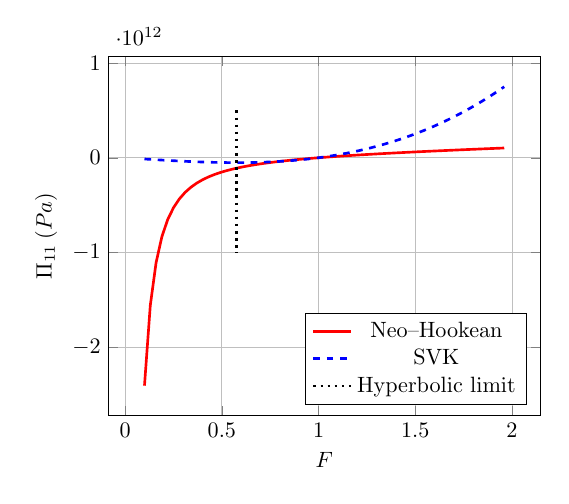
\begin{tikzpicture}[scale=0.8]
\begin{axis}[xlabel=$F$,ylabel=$\Pi_{11} \:(Pa)$,ymajorgrids=true,xmajorgrids=true,legend pos=south east]
\addplot[Red,very thick] coordinates {(0.1,-2408422023218.795) (0.13,-1561400030186.036) (0.15999999999999998,-1108128415709.1655) (0.18999999999999995,-833911946074.9946) (0.21999999999999995,-653670173462.2463) (0.24999999999999992,-527854249959.5669) (0.2799999999999999,-435915059061.98395) (0.30999999999999994,-366257400931.6964) (0.33999999999999986,-311907911555.59503) (0.3699999999999999,-268454254884.53748) (0.3999999999999998,-232986311465.25177) (0.4299999999999998,-203517286416.10312) (0.45999999999999985,-178650539697.26926) (0.48999999999999977,-157379384667.57828) (0.5199999999999998,-138962278617.30313) (0.5499999999999998,-122842502435.93149) (0.5799999999999997,-108595017949.65054) (0.6099999999999998,-95890438067.54034) (0.6399999999999997,-84470064152.38515) (0.6699999999999997,-74128253013.84497) (0.6999999999999996,-64699742636.182884) (0.7299999999999996,-56050397620.76282) (0.7599999999999997,-48070354307.61169) (0.7899999999999996,-40668876630.01929) (0.8199999999999996,-33770449303.23107) (0.8499999999999996,-27311777895.064568) (0.8799999999999996,-21239461747.10439) (0.9099999999999996,-15508171775.6262) (0.9399999999999996,-10079211097.636282) (0.9699999999999995,-4919368770.523872) (0.9999999999999996,-7.686159401251085e-05) (1.0299999999999996,4703717188.049879) (1.0599999999999996,9213386680.69596) (1.0899999999999996,13547889345.500956) (1.1199999999999997,17723790714.211426) (1.1499999999999995,21755678576.81564) (1.1799999999999995,25656444006.788513) (1.2099999999999995,29437516460.917877) (1.2399999999999995,33109061386.49867) (1.2699999999999996,36680147058.33992) (1.2999999999999994,40158886035.87196) (1.3299999999999994,43552555586.440025) (1.3599999999999994,46867700597.432465) (1.3899999999999995,50110221846.80901) (1.4199999999999995,53285451980.78061) (1.4499999999999995,56398221129.891785) (1.4799999999999993,59452913758.40091) (1.5099999999999993,62453518069.58127) (1.5399999999999994,65403669068.15871) (1.5699999999999994,68306686200.273705) (1.5999999999999994,71165606343.04538) (1.6299999999999992,73983212793.691) (1.6599999999999993,76762060807.20117) (1.6899999999999993,79504500147.80951) (1.7199999999999993,82212695049.75154) (1.7499999999999993,84888641924.53296) (1.7799999999999994,87534185103.07764) (1.8099999999999992,90151030860.04399) (1.8399999999999992,92740759932.94342) (1.8699999999999992,95304838719.37517) (1.8999999999999992,97844629310.81384) (1.9299999999999993,100361398500.2192) (1.959999999999999,102856325882.67926) };
\addplot[Blue,very thick,dashed] coordinates {(0.1,-13326923076.923077) (0.13,-17204250000.0) (0.15999999999999998,-20987076923.076923) (0.18999999999999995,-24653596153.846146) (0.21999999999999995,-28181999999.999992) (0.24999999999999992,-31550480769.23076) (0.2799999999999999,-34737230769.23076) (0.30999999999999994,-37720442307.69231) (0.33999999999999986,-40478307692.30768) (0.3699999999999999,-42989019230.76922) (0.3999999999999998,-45230769230.76922) (0.4299999999999998,-47181749999.99999) (0.45999999999999985,-48820153846.15384) (0.48999999999999977,-50124173076.923065) (0.5199999999999998,-51071999999.99999) (0.5499999999999998,-51641826923.07693) (0.5799999999999997,-51811846153.846146) (0.6099999999999998,-51560250000.00001) (0.6399999999999997,-50865230769.23079) (0.6699999999999997,-49704980769.23078) (0.6999999999999996,-48057692307.69232) (0.7299999999999996,-45901557692.30772) (0.7599999999999997,-43214769230.76926) (0.7899999999999996,-39975519230.76928) (0.8199999999999996,-36162000000.00005) (0.8499999999999996,-31752403846.153904) (0.8799999999999996,-26724923076.92316) (0.9099999999999996,-21057750000.000076) (0.9399999999999996,-14729076923.07701) (0.9699999999999995,-7717096153.846271) (0.9999999999999996,-0.0001195624795750168) (1.0299999999999996,8444019230.769098) (1.0599999999999996,17636769230.76912) (1.0899999999999996,27600057692.30757) (1.1199999999999997,38355692307.692184) (1.1499999999999995,49925480769.23054) (1.1799999999999995,62331230769.230545) (1.2099999999999995,75594749999.99979) (1.2399999999999995,89737846153.84596) (1.2699999999999996,104782326923.07669) (1.2999999999999994,120749999999.99965) (1.3299999999999994,137662673076.92273) (1.3599999999999994,155542153846.15347) (1.3899999999999995,174410249999.99966) (1.4199999999999995,194288769230.7689) (1.4499999999999995,215199519230.7689) (1.4799999999999993,237164307692.3072) (1.5099999999999993,260204942307.69174) (1.5399999999999994,284343230769.2303) (1.5699999999999994,309600980769.2303) (1.5999999999999994,335999999999.9995) (1.6299999999999992,363562096153.84546) (1.6599999999999993,392309076923.07623) (1.6899999999999993,422262749999.99927) (1.7199999999999993,453444923076.9223) (1.7499999999999993,485877403846.15314) (1.7799999999999994,519581999999.99927) (1.8099999999999992,554580519230.7682) (1.8399999999999992,590894769230.7683) (1.8699999999999992,628546557692.3066) (1.8999999999999992,667557692307.6913) (1.9299999999999993,707949980769.2297) (1.959999999999999,749745230769.2295) };
\addplot[dotted,very thick] coordinates { (sqrt(1./3),0.5e12) (sqrt(1./3),-1.e12)};
\legend{Neo--Hookean,SVK,Hyperbolic limit}
\end{axis}
\end{tikzpicture}
 \phantomsubcaption \label{subfig:SVK_NH_Pi}}
    {\definecolor{Red}{RGB}{217,33,32}
\definecolor{Blue}{RGB}{63,96,174}
\definecolor{Duck}{RGB}{83,158,182}
\definecolor{Green}{RGB}{109,179,136}
\definecolor{Yellow}{RGB}{202,184,67}
\definecolor{Orange}{RGB}{231,133,50}
\definecolor{Red}{RGB}{217,33,32}
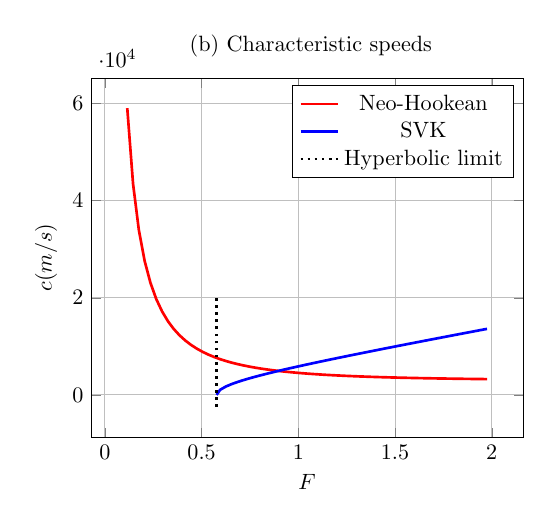
\begin{tikzpicture}[scale=0.8]
\begin{axis}[xlabel=$F$,ylabel=$\abs{c} (m/s)$,ymajorgrids=true,xmajorgrids=true,title={\normalsize{ (b) Characteristic speeds}}]
\addplot[Red,very thick] coordinates {(0.11547005383792518,59012.035730808406) (0.14547005383792516,43444.15680640866) (0.17547005383792513,33909.66271892359) (0.20547005383792513,27551.616086072518) (0.23547005383792513,23052.45426344622) (0.2654700538379251,19726.297080765253) (0.2954700538379251,17183.410876622853) (0.3254700538379251,15187.108927674422) (0.35547005383792507,13585.92851121213) (0.38547005383792504,12278.756336822797) (0.415470053837925,11195.691489974464) (0.44547005383792504,10286.970773511453) (0.475470053837925,9516.269220270638) (0.505470053837925,8856.492138358943) (0.535470053837925,8287.045413546242) (0.5654700538379249,7792.014425579814) (0.595470053837925,7358.918900548452) (0.625470053837925,6977.8428382999955) (0.6554700538379249,6640.81463208358) (0.6854700538379249,6341.3576871839605) (0.7154700538379248,6074.159484360366) (0.7454700538379249,5834.824367261866) (0.7754700538379249,5619.6864514897625) (0.8054700538379248,5425.666332338412) (0.8354700538379248,5250.16012367266) (0.8654700538379249,5090.952654625974) (0.8954700538379248,4946.148920983796) (0.9254700538379248,4814.119475233549) (0.9554700538379248,4693.456563660641) (0.9854700538379247,4582.938625301644) (1.0154700538379247,4481.501352586511) (1.0454700538379247,4388.21394243672) (1.0754700538379247,4302.259484218307) (1.1054700538379247,4222.918668359039) (1.1354700538379248,4149.556178447647) (1.1654700538379246,4081.609265724866) (1.1954700538379246,4018.57810915085) (1.2254700538379246,3960.0176447237714) (1.2554700538379246,3905.530610294456) (1.2854700538379247,3854.761601089376) (1.3154700538379245,3807.391969723345) (1.3454700538379245,3763.135435049281) (1.3754700538379245,3721.7342885593334) (1.4054700538379246,3682.9561065868374) (1.4354700538379246,3646.590892305437) (1.4654700538379246,3612.448584281259) (1.4954700538379244,3580.3568787248346) (1.5254700538379244,3550.1593210921387) (1.5554700538379245,3521.7136296737963) (1.5854700538379245,3494.8902195829423) (1.6154700538379245,3469.5709003379666) (1.6454700538379243,3445.6477242208375) (1.6754700538379244,3423.021965921998) (1.7054700538379244,3401.6032167766175) (1.7354700538379244,3381.308579249105) (1.7654700538379244,3362.061949309672) (1.7954700538379245,3343.793376030597) (1.8254700538379243,3326.438489161275) (1.8554700538379243,3309.9379866615427) (1.8854700538379243,3294.237175216221) (1.9154700538379243,3279.2855576483526) (1.9454700538379244,3265.0364619174256) (1.9754700538379242,3251.446707051308) };
\addplot[Blue,very thick] coordinates {(sqrt(1./3.),0.) (0.595470053837925,1048.9455179543422) (0.625470053837925,1731.1029259571128) (0.6554700538379249,2233.012146664284) (0.6854700538379249,2658.790029377158) (0.7154700538379248,3040.5889001561395) (0.7454700538379249,3393.286396027051) (0.7754700538379249,3725.1576526965905) (0.8054700538379248,4041.336632315833) (0.8354700538379248,4345.250197655363) (0.8654700538379249,4639.309436869055) (0.8954700538379248,4925.279696432755) (0.9254700538379248,5204.494537554574) (0.9554700538379248,5477.987035494905) (0.9854700538379247,5746.574266198714) (1.0154700538379247,6010.9138156437175) (1.0454700538379247,6271.542813975518) (1.0754700538379247,6528.905643538706) (1.1054700538379247,6783.374072186155) (1.1354700538379248,7035.262182069363) (1.1654700538379246,7284.837637447764) (1.1954700538379246,7532.330323596269) (1.2254700538379246,7777.939063134427) (1.2554700538379246,8021.836903239133) (1.2854700538379247,8264.175324905573) (1.3154700538379245,8505.087628335128) (1.3454700538379245,8744.691681060722) (1.3754700538379245,8983.092167747032) (1.4054700538379246,9220.382446402957) (1.4354700538379246,9456.646090866763) (1.4654700538379246,9691.958181097758) (1.4954700538379244,9926.386389147965) (1.5254700538379244,10159.991898394823) (1.5554700538379245,10392.830185782268) (1.5854700538379245,10624.951690800193) (1.6154700538379245,10856.402390269113) (1.6454700538379243,11087.224294354115) (1.6754700538379244,11317.455876364773) (1.7054700538379244,11547.132446624275) (1.7354700538379244,11776.286478876727) (1.7654700538379244,12004.947896244235) (1.7954700538379245,12233.144322567889) (1.8254700538379243,12460.901304010209) (1.8554700538379243,12688.242505014787) (1.8854700538379243,12915.189882077482) (1.9154700538379243,13141.763838254037) (1.9454700538379244,13367.983360890252) (1.9754700538379242,13593.866144695845) };
\addplot[dotted,very thick] coordinates {(sqrt(1./3.),-0.25e4) (sqrt(1./3.),2.e4)};
\legend{Neo-Hookean,SVK,Hyperbolic limit}
\end{axis}
\end{tikzpicture}
 \phantomsubcaption \label{subfig:SVK_NH_speeds}}
    \caption{Comparison of neo-Hookean and Saint-Venant-Kirchhoff hyperelastic models.}
    \label{fig:SVK-NH}
  \end{figure}
  At last, figure \ref{fig:SVK-NH}\subref{subfig:SVK_NH_Pi} shows the non-physical behaviour of Saint-Venant-Kirchhoff model for high compression loads that lead to a stress tensor tending to zero.
\end{remark}

\todo[inline]{comment the elastoviscoplastic case ?}
%%% Local Variables:
%%% mode: latex
%%% TeX-master: "../mainManuscript"
%%% End:
